%% -*- coding:sjis -*-
%%
%% 2013-07-18, Koichi Murase, 入力
%%
\begin{question}{第1問}{村瀬}
\begin{enumerate}
\item
  3次元空間回転を表す3次元実正方行列すべての集合を$R$とする。$R$は単位行列$I$も
  含むものとする。これに関して、以下の各命題の真偽を○(真)か×(偽)かで答えよ。
  \begin{enumerate}
    \def\theenumii{\alph{enumii}}
    \def\labelenumii{(\theenumii)}
  \item $X\in R$かつ$Y\in R$ならば$XY\in R$である。
  \item $X\in R$かつ$Y\in R$ならば$XY=YX$である。
  \item $X\in R$ならば$^tXX=X^tX=I$である。ただし、$^tX$は$X$の転置行列を表す。
  \item $^tXX=X^tX=I$であるならば$X\in R$である。
  \item $X\in R$ならば$U^\dag XU$が対角行列であるようなユニタリ行列$U$が存在する。た
    だし、$U^\dag$は$U$のエルミート共役行列(転置行列の複素共役)を表す。
  \end{enumerate}
\item
  $\Omega(\bm{n},\theta)$を、単位ベクトル$\bm{n}$の方向を回転軸とした角度$\theta$の回転を表す3次元実正方行
  列とする。ここで、$\bm{n}$方向に右ねじを進める時右ねじを回す向きを正とする回転角を
  $\theta$とする。また、任意の3次元実ベクトル$\bm{v}_0$に対して、$\bm{v}(\theta)$を$\bm{v}(\theta)=\Omega(\bm{n},\theta)\bm{v}_0$で
  定義する。以下の設問に答えよ。
  \begin{enumerate}
  \item
    $\bm{n}=(0,0,1)$のとき、$\Omega(\bm{n},\theta)$の3つの固有値を答えよ。
  \item
    任意の$\bm{n}$に対して、$\Omega(\bm{n},\theta)$の3つの固有値を答えよ。
  \item\ilabel{A1.2.3}
    原点を始点としたとき$\bm{v}(\theta)$の終点がどれだけ移動するかを考えて、
    \begin{align*}
      \bm{v}(\theta+\Delta\theta) - \bm{v}(\theta)
        = \bm{n}\times\bm{v}(\theta)\Delta\theta
    \end{align*}
    となることを説明せよ。ただし、$\Delta\theta$は$\theta$に比べて十分小さいものとする。また、
    $\times$はベクトル積(外積)である。必要なら図を用いて説明してもよい。
  \item\ilabel{A1.2.4}
    設問\iref{A1.2.3}の結果から得られる$\bm{v}(\theta)$に関する微分方程式を解くことによって、
    \begin{align*}
      \Omega(\bm{n},\theta) = e^{\theta A(\bm{n})}
    \end{align*}
    であることを示せ。ここで、$A(\bm{a})$は、ある3次元実ベクトル$\bm{a}$に対して決まる
    3次元実正方行列であり、任意のベクトル$\bm{u}$に対して$A(\bm{a})\bm{u}=\bm{a}\times\bm{u}$を満たす
    ものとする。
  \item
    3次元実交代行列
    \begin{align*}
      X = \begin{pmatrix}
        0 & x_{12} & x_{13} \\
        x_{21} & 0 & x_{23} \\
        x_{31} & x_{32} & 0
      \end{pmatrix}\quad\quad\mbox{(ただし、$x_{ij}=-x_{ji},\quad i,j=1,\ldots,3$)}
    \end{align*}
    に対して、$X=A(\bm{a}_0)$となるような3次元実ベクトル$\bm{a}_0$を求めよ。ここで、$A$
    は設問\iref{A1.2.4}で定義されたものと同じである。
  \item
    $Y=e^X$ となるような3次元実交代行列 $X$ が存在するならば $Y$ は3次元回転を
    表す行列であることを示せ。
  \end{enumerate}
\end{enumerate}
\end{question}

\begin{question}{第2問}{村瀬}
$n=0,1,2,\ldots$ に対して、関数$f_n(x)$を
\begin{align*}
  f_n(x) = e^{x^2} \frac{d^n}{dx^n}(e^{-x^2})
\end{align*}
と定義する。以下の設問に答えよ。
\begin{enumerate}
\item
  $f_n(x)$は$x$の多項式である。$x$の何次の多項式であるか答えよ。

\item
  $n>1$に対して、
  \begin{align*}
    \int_{-\infty}^{\infty} x f_n(x) e^{-x^2}dx
  \end{align*}
  を求めよ。

\item
  一般の$n$に対して、
  \begin{align*}
    \int_{-\infty}^{\infty} x^n f_n(x) e^{-x^2} dx
  \end{align*}
  を求めよ。ただし、必要であれば、
  \begin{align*}
    \int_{-\infty}^{\infty} e^{-x^2}dx = \sqrt{\pi}
  \end{align*}
  を用いてよい。

\item\ilabel{A2.4}
  $z$を複素数とするとき、
  \begin{align*}
    e^{-z^2} = \frac1{2\pi\i}\oint_C\frac{e^-\omega^2}{\omega-z}d\omega
  \end{align*}
  が成り立つ。ここで、複素平面上の積分経路$C$は、図1のような$z$を中心とした半径
  1の反時計回りの円周であるとする。このことを用いて、
  \begin{align*}
    \sum_{n=0}^\infty \frac{t^n}{n!} f_n(z) = e^{-t^2-2zt}\quad(|t|<1)
  \end{align*}
  となることを示せ。ただし、今の場合、無限級数和と積分の順序を入れ替えてもよい。

\item
  設問\iref{A2.4}で得られた関数$e^{-t^2-2tz}$は、
  \begin{align*}
    \frac{\partial^2}{\partial z^2} e^{-t^2-2tz}
    - 2z \frac{\partial}{\partial z} e^{-t^2-2tz}
    = -2t\frac{\partial}{\partial t} e^{-t^2-2tz}
  \end{align*}
  という式を満たす。このことを用いて、関数$f_n(z)$が
  \begin{align*}
    \frac{d^2}{dz^2} f_n(z)
    - 2z \frac{d}{dz} f_n(z) + \lambda f_n(z) = 0
  \end{align*}
  という微分方程式を満たすということを示し、そのときの$\lambda$を求めよ。
\end{enumerate}
\begin{center}
  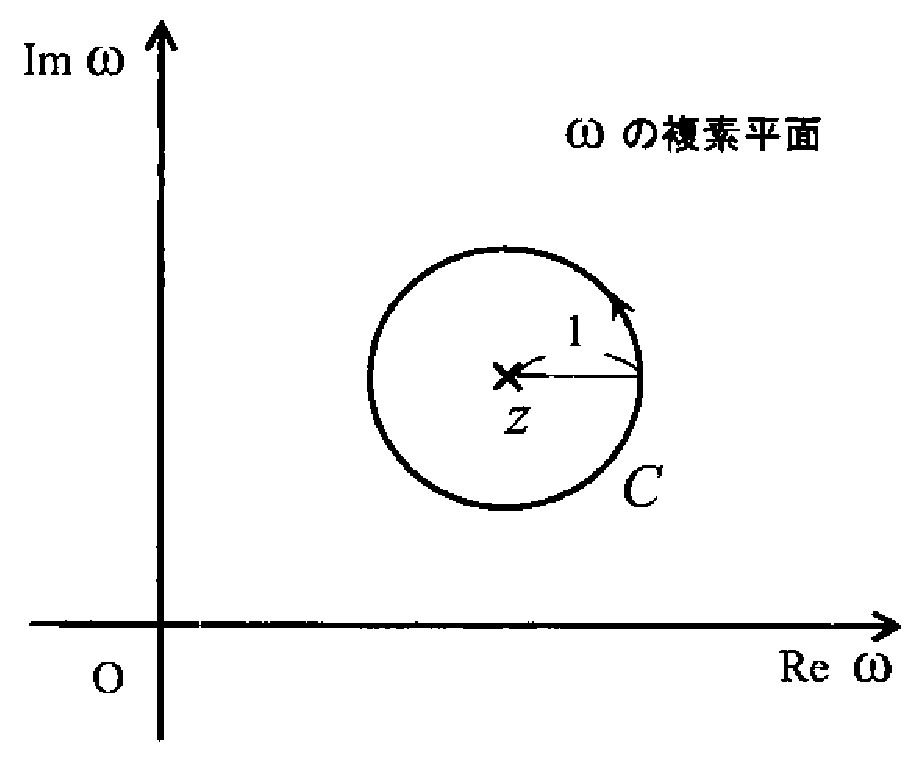
\includegraphics[width=0.6\textwidth]{2007mathQ2_1r.eps}\\図1: 積分経路 $C$
\end{center}
\end{question}
